%%%%%%%%%%%%%%%%%%%%%%%%%%%%%%%%%%%%%%%%%%
% Mathematics Final Year Research Projects
% LaTeX Template
% Version 1.0 (31/01/24)
%%%%%%%%%%%%%%%%%%%%%%%%%%%%%%%%%%%%%%%%%%

\documentclass[a4paper,11pt, titlepage]{article}

%% Language and font encodings
\usepackage[english]{babel}
\usepackage[utf8]{inputenc}
\usepackage[T1]{fontenc}

%% Sets page size and margins
\usepackage[a4paper,top=1in,bottom=1in,left=1in,right=1in,marginparwidth=1.75cm]{geometry}

%% Useful packages
\usepackage{afterpage}
\usepackage{amsmath}
\usepackage{amsthm}
\usepackage{amssymb}
\usepackage{csquotes}
\usepackage{enumitem}
\usepackage{graphicx}
\usepackage{lipsum}
\usepackage{booktabs}
\usepackage{caption}
\usepackage{placeins}

\captionsetup[figure]{labelfont={bf},name={Figure},labelsep=quad}
\captionsetup[table]{labelfont={bf},name={Table},labelsep=quad}

\usepackage{bm}
\usepackage[normalem]{ulem}

\usepackage[colorinlistoftodos]{todonotes}
\usepackage[colorlinks=true, allcolors=blue]{hyperref}

\renewcommand*{\rmdefault}{bch}
\renewcommand*{\ttdefault}{lmtt}

\DeclareMathOperator*{\argmin}{\arg\!\min}
\DeclareMathOperator*{\argmax}{\arg\!\max}

\setlength{\parskip}{0.5em}

\usepackage[numbers, comma, square, sort&compress]{natbib}
\bibliographystyle{abbrvnat}

\theoremstyle{definition}
\newtheorem{definition}{Definition}[section]
\theoremstyle{plain}
\newtheorem{theorem}{Theorem}[section]
\newtheorem{corollary}{Corollary}[theorem]
\newtheorem{lemma}[theorem]{Lemma}
\theoremstyle{remark}
\newtheorem*{remark}{Remark}

\begin{document}

\subsection{Method 4: Monte Carlo Simulation}

Monte Carlo Simulation tackles this problem by simulating $M$ independent paths of the terminal stock price under the risk-neutral assumption using the Geometric Brownian Motion equation under the Black-Scholes framework \cite{black1973}:

\begin{equation}
    S_T^{(m)} = S_0 \exp \left( \left( r - \frac{1}{2}\sigma^2 \right) T + \sigma W_{T-0}^{(m)} \right), \quad W_{T-0}^{(m)} \sim \mathcal{N}(0,T)
\end{equation}

The approximated option price $\hat{C}(0, S_0)$ can be estimated with the continuous discounted average of the simulated payoffs:

\begin{equation}
    \hat{C}(0, S_0) = e^{-rT} \frac{1}{M} \sum_{m=1}^{M} (S_T^{(m)} - K)^+
\end{equation}

where $e^{-rT}$ is the continuous discount factor, and result of Monte Carlo simulation is the mean of all discounted simulated price.

\subsubsection{Statistical Convergence and Confidence Intervals}

Because the Monte Carlo method relies on random sampling, our calculated price $\hat{C}$ is a statistical estimator. To measure the precision of the estimate, we could calculate the standard error (SE) of the discounted payoffs.

By the Central Limit Theorem and Slutsky lemma, as the number of simulations $M$ becomes large, the distribution of our estimator approaches a normal distribution. Therefore, we can construct a 95\% Confidence Interval (C.I.) for the true option price:

\begin{equation}
    \hat{\sigma} = \sqrt{\frac{1}{M-1}\sum_{m=1}^{M} \left(C_m - \hat{C}\right)^2} \overset{p}{\longrightarrow} \sigma
\end{equation}

\begin{equation}
    \frac{\hat{C} - C}{\hat{\sigma}/\sqrt{M}} \sim \mathcal{N}(0, 1) \implies 95\% \text{ C.I.} = \left[ \hat{C} - \frac{1.96\,\hat{\sigma}}{\sqrt{M}}, \; \hat{C} + \frac{1.96\,\hat{\sigma}}{\sqrt{M}} \right]
\end{equation}

where $C$ is the true option price, $C_m = e^{-rT}(S_T^{(m)} - K)^+$ is the $m$-th discounted payoff, $\hat{\sigma}$ is their sample standard deviation, and $SE = \hat{\sigma}/\sqrt{M}$ is the standard error of the estimate.

Since $SE = \hat{\sigma}/\sqrt{M}$, the half-width of the confidence interval shrinks at rate $\mathcal{O}(M^{-1/2})$. This is the fundamental convergence rate of Monte Carlo, reducing the error requires quadratically more simulations. To halve the estimation error from a baseline of $M_1$ paths, the required $M_2$ must satisfy:

\begin{equation}
\frac{\hat{\sigma}}{\sqrt{M_2}} = \frac{1}{2} \left( \frac{\hat{\sigma}}{\sqrt{M_1}} \right) \implies \frac{1}{M_2} = \frac{1}{4M_1} \implies M_2 = 4M_1
\end{equation}

Figure~\ref{fig:mc_convergence} demonstrates this empirically, showing how the mean absolute error $|\hat{C} - C_{BS}|$ decays as $M$ grows, closely tracking the theoretical $\mathcal{O}(M^{-1/2})$ reference.

\begin{figure}[htbp]
    \centering
    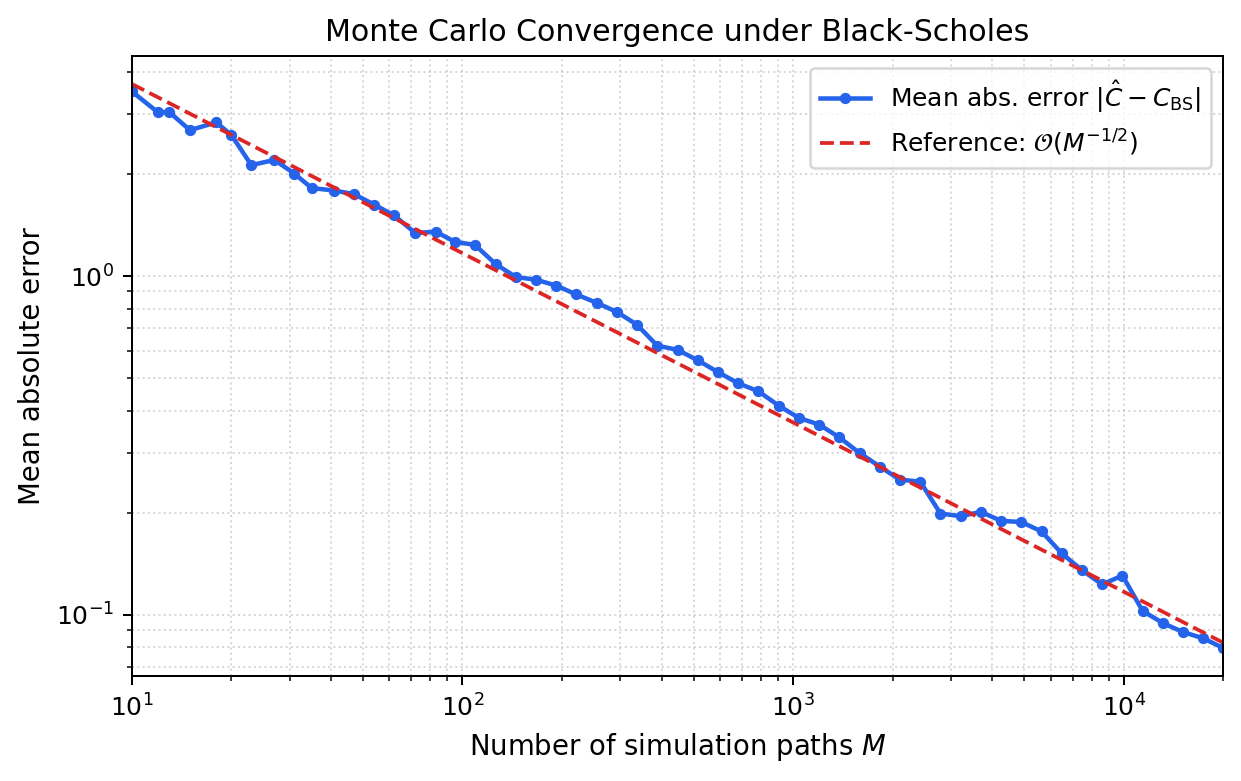
\includegraphics[width=0.9\textwidth]{figures/mc_convergence_plot.png}
    \caption{Convergence of the Monte Carlo estimator against the Black-Scholes closed-form price as a function of the number of simulation paths $M$, with parameters $S_0 = K = 100$, $T = 1$, $r = 0.05$, $\sigma = 0.2$. Each point is the mean absolute error over 50 independent trials. The dashed line shows the theoretical $\mathcal{O}(M^{-1/2})$ reference.}
    \label{fig:mc_convergence}
\end{figure}

\subsubsection{Numerical Validation}

To verify the estimator, we compare the Monte Carlo price ($M = 10^4$ paths) against the Black-Scholes closed-form across different market conditions. Options are typically classified by their \textit{moneyness}, the relationship between the current asset price $S_0$ and the strike $K$. An option is \textit{in-the-money} (ITM) when $S_0 > K$, meaning it would have positive intrinsic value if exercised immediately; \textit{at-the-money} (ATM) when $S_0 \approx K$; and \textit{out-of-the-money} (OTM) when $S_0 < K$, where immediate exercise would be worthless.

Table~\ref{tab:mc_validation} summarises five representative cases, all with $r = 0.05$ and $T = 1$.

\begin{table}[htbp]
\centering
\caption{Monte Carlo vs.\ Black-Scholes closed-form European call prices for $M = 10^4$ paths, $r = 0.05$, $T = 1$.}
\label{tab:mc_validation}
\begin{tabular}{lccccccccc}
\toprule
Scenario & $S_0$ & $K$ & $\sigma$ & BS Price & MC Price & 95\% CI & SE & Abs Err & \% Err \\
\midrule
Deep ITM     & 120 & 100 & 0.2 & 26.1690 & 26.0162 & $[25.58,\ 26.46]$ & 0.2246 & 0.1529 & 0.58 \\
ATM          & 100 & 100 & 0.2 & 10.4506 & 10.3452 & $[10.06,\ 10.63]$ & 0.1477 & 0.1054 & 1.01 \\
Slight OTM   &  95 & 100 & 0.2 &  7.5109 &  7.4351 & $[\ 7.19,\ \ 7.68]$ & 0.1251 & 0.0758 & 1.01 \\
Deep OTM     &  80 & 100 & 0.2 &  1.8594 &  1.8712 & $[\ 1.75,\ \ 1.99]$ & 0.0595 & 0.0118 & 0.63 \\
High vol ATM & 100 & 100 & 0.5 & 21.7926 & 21.6259 & $[20.81,\ 22.44]$ & 0.4153 & 0.1667 & 0.76 \\
\bottomrule
\end{tabular}
\end{table}

Across all cases the percentage error stays below 1.1\%, showing that $M = 10^4$ paths gives a reliable approximation throughout different moneyness regimes. The high volatility ATM case stands out with the widest CI (width $\approx 1.63$) and the largest standard error ($SE = 0.415$); higher volatility increases the dispersion of the terminal payoffs, so more paths are needed to achieve the same precision. The deep OTM case, by contrast, has the narrowest CI despite a small absolute option value, because most paths expire worthless and the payoff variance is low.

\FloatBarrier
\subsection{Method 5: Deep Neural Network Pricing}
\label{sec:dnn_bs}

\subsubsection{Motivation: Why Train a Network at All?}

Every method we have used so far (closed-form formulas, Monte Carlo simulation, finite-difference / PDE solvers) runs into the same wall as soon as the model gets richer: the cost of pricing grows very quickly with the number of state variables and parameters involved. The Black-Scholes PDE that prices a European call is a function of just two variables, the asset price $S$ and time $t$; discretising each on a grid of $N$ points costs roughly $\mathcal{O}(N^2)$ to solve, perfectly manageable for $N$ in the hundreds.

The moment we move to a model with stochastic volatility, exactly the extension this project is built around, the variance $V_t$ stops being a fixed parameter $\sigma$ and becomes a third state variable that the PDE has to track alongside $S$ and $t$, governed by its own dynamics: a mean-reversion speed $\kappa$, a long-run level $\theta$, a vol-of-vol $\omega$, and a correlation $\rho$ with the asset. Adding just this one extra dimension turns an $\mathcal{O}(N^2)$ grid into an $\mathcal{O}(N^3)$ one: with $N = 100$ points per axis, the two-dimensional Black-Scholes solve needs $10^4$ grid nodes, while the three-dimensional version (with, say, $\kappa$ as the new axis) needs $10^6$, a hundred-fold jump from introducing a single new parameter. Let $\theta$, $\omega$ or $\rho$ vary too, and the grid size keeps multiplying by a further factor of $N$ each time. This is the curse of dimensionality, and it is why classical PDE grids (and, to a lesser extent, Monte Carlo, where variance reduction also gets harder in higher dimensions) become unworkable almost as soon as the model becomes interesting enough to be worth using.

A trained neural network sidesteps this problem entirely, because it never discretises the input space at all; this is precisely the meshfree idea behind the Deep Galerkin Method of \cite{sirignano2018}, who train networks to satisfy a PDE's differential operator directly on randomly sampled points rather than on a grid and report accurate solutions to PDE problems in up to 200 dimensions. Rather than representing the price as values on a grid, it represents the pricing function as a fixed, finite collection of weights, and the number of weights depends only on the network's width and depth, not on how finely we would otherwise have to grid up the parameter space. For a network with two hidden layers of $n$ neurons each and an input dimension $d$, counting the weights and biases layer by layer gives
\[
P(d, n) = \underbrace{(d+1)n}_{\text{layer 1}} + \underbrace{(n+1)n}_{\text{layer 2}} + \underbrace{(n+1)}_{\text{output}} = n^2 + (d+3)n + 1 .
\]
This grows \emph{linearly} in $d$: doubling the number of input parameters roughly doubles the number of weights, not the size of the network squared or cubed. Concretely, $P(5, 20) = 561$ for the Black-Scholes network described below, and $P(9, 40) = 2{,}081$ for the nine-input Heston network later in this chapter, both perfectly trainable on a laptop in well under a minute, however large $d$ becomes.

This is not a free lunch, and it is worth being upfront about where the approach is weakest; these also strike us as the most natural directions for any follow-up work. First, the network only ever sees the parameter ranges and the single (synthetic) underlying it was trained on; it has learned a surrogate for \emph{those} ranges, and there is no guarantee it generalises to a very different stock, a very different rate environment, or a period of unusual market stress. Second, as the next few subsections show in detail, the network is systematically weaker at pricing deep out-of-the-money options, where the true price is tiny and even a small absolute error becomes a huge relative one. Third, the network is trained entirely on simulated prices, $500{,}000$ of them, whereas real, traded option prices are comparatively scarce, noisier, and shaped by frictions (bid-ask spreads, discrete strike grids, liquidity effects) that a model trained purely on theoretical prices never has to contend with. And finally, both the Black-Scholes and the Heston formulas we are approximating are themselves models of a market that has moved on a great deal since Black and Scholes derived their original formula in 1973 \cite{black1973}; volatility surfaces, correlation structures, and the very stylised facts that motivate stochastic volatility in the first place have all evolved since then. A DNN surrogate is, at best, only ever as faithful as the pricing model it has been trained to imitate.

\subsubsection{Generating the Training Data}

To train a surrogate we first need a large supervised dataset of (parameters $\to$ price) pairs. We draw $500{,}000$ parameter combinations $(S, K, T, r, \sigma)$ via uniform random sampling over realistic ranges, $S, K \in [50, 200]$, $T \in [0.05, 3.0]$, $r \in [0, 0.10]$ and $\sigma \in [0.05, 0.80]$, and label each one with the \emph{exact} Black-Scholes closed-form price $C_{BS}(S, K, T, r, \sigma)$. Using the closed-form price rather than, say, a Monte Carlo estimate is a deliberate choice: it gives us noise-free labels, so any error the network later makes is attributable to the network itself and not to randomness inherited from the label-generation process, exactly the clean, large training set a DNN needs in order to learn a smooth pricing surface well.

\subsubsection{Parameter Normalisation}

Before any of this reaches the network, we rescale every input. The five parameters live on very different numerical scales: $S$ and $K$ range over $[50, 200]$, $T$ over $[0.05, 3.0]$, $r$ over $[0, 0.10]$, and $\sigma$ over $[0.05, 0.80]$. Fed to the network as-is, $S$ and $K$ would dominate purely because their raw values are an order of magnitude larger than $r$'s; the network would have to spend its first few layers learning to "undo" this scale mismatch before it could learn anything about the actual pricing relationship, and gradient descent converges far more slowly, and less reliably, when inputs sit on such different scales.

We fix this with the standard $z$-score normalisation: for each feature $x_j$ we compute the training-set mean $\mu_j$ and standard deviation $s_j$, and replace every value with
\[
x_j' = \frac{x_j - \mu_j}{s_j} .
\]
After this transform every input has (approximately) zero mean and unit variance, so no feature dominates simply because of its raw scale, and the loss surface the optimiser navigates is much better conditioned. Crucially, $\mu_j$ and $s_j$ are estimated only from the training split and then applied unchanged to the validation and test splits; fitting the scaler on data the network will later be evaluated on would leak information from the test set into training.

\subsubsection{Network Architecture}

The surrogate, \texttt{OptionPricingDNN}, is a small feedforward network: an input layer of dimension $d = 5$, two hidden layers of $n = 20$ neurons each with ReLU activations $\ell(\cdot) = \max(0, \cdot)$, and a single linear output neuron giving the price. Writing $x = (S, K, T, r, \sigma)$ for the normalised input, the forward pass is
\[
z_1 = A_1 x + b_1, \quad \tilde z_1 = \ell(z_1), \qquad
z_2 = A_2 \tilde z_1 + b_2, \quad \tilde z_2 = \ell(z_2), \qquad
\hat C = A_3 \tilde z_2 + b_3,
\]
with $A_1 \in \mathbb{R}^{20 \times 5}$, $A_2 \in \mathbb{R}^{20 \times 20}$, $A_3 \in \mathbb{R}^{1 \times 20}$, and matching bias vectors $b_1, b_2, b_3$. Counting weights and biases layer by layer,
\[
\underbrace{(5 \times 20 + 20)}_{\text{layer 1: } 120} + \underbrace{(20 \times 20 + 20)}_{\text{layer 2: } 420} + \underbrace{(20 \times 1 + 1)}_{\text{output: } 21} = 561
\]
trainable parameters in total, exactly the $P(5, 20) = 561$ predicted by the formula above. Weights are initialised with He (Kaiming) normal initialisation, the natural choice for ReLU networks since it keeps the variance of activations roughly constant from one layer to the next.

The choice of just two modest hidden layers is not arbitrary. By the universal approximation theorem for networks with non-polynomial activation functions \cite{leshno1993}, a feedforward network with even a single hidden layer can approximate any continuous function on a compact set arbitrarily well, provided it is given enough neurons. The Black-Scholes pricing function $C_{BS}$ is smooth and well-behaved on the (compact) ranges we sample from, so there is good theoretical justification for expecting a network of this size to be more than capable of representing it; the only remaining question is whether training can actually \emph{find} the right weights, which is what the rest of this section investigates.

\subsubsection{Training}

We split the $500{,}000$ labelled examples $80/20$ into a training and a held-out test set, then reserve a further $10\%$ of the training set for validation, leaving roughly $349{,}000$ examples for the optimiser to learn from. The network is trained to minimise the mean squared error between its prediction and the true closed-form price,
\[
\mathcal{L} = \frac{1}{B}\sum_{i=1}^{B}\left(\hat C_i - C_i\right)^2,
\]
averaged over mini-batches of $B = 4096$ examples. We use the Adam optimiser \cite{kingma2015} with an initial learning rate of $10^{-3}$ (small enough that the network does not overshoot and oscillate around the minimum, but large enough to make visible progress within a modest number of epochs) together with a \texttt{ReduceLROnPlateau} scheduler that halves the learning rate whenever the validation loss fails to improve for five consecutive epochs. We train for $60$ epochs and, at the end, restore the weights from whichever epoch achieved the lowest validation loss rather than simply keeping the final epoch's weights.

\subsubsection{Loss Curves}

Figure~\ref{fig:dnn_bs_loss} shows the training and validation MSE over the $60$ epochs, plotted on a normal (linear) scale with the gridlines removed. The original log-scaled, gridded version made the curves harder to read than they needed to be: both losses fall sharply within the first handful of epochs and then flatten out, and a logarithmic axis stretches out this early, uninteresting transient at the expense of the part of the plot that actually matters, whether training and validation continue to track one another once they level off.

\begin{figure}[htbp]
    \centering
    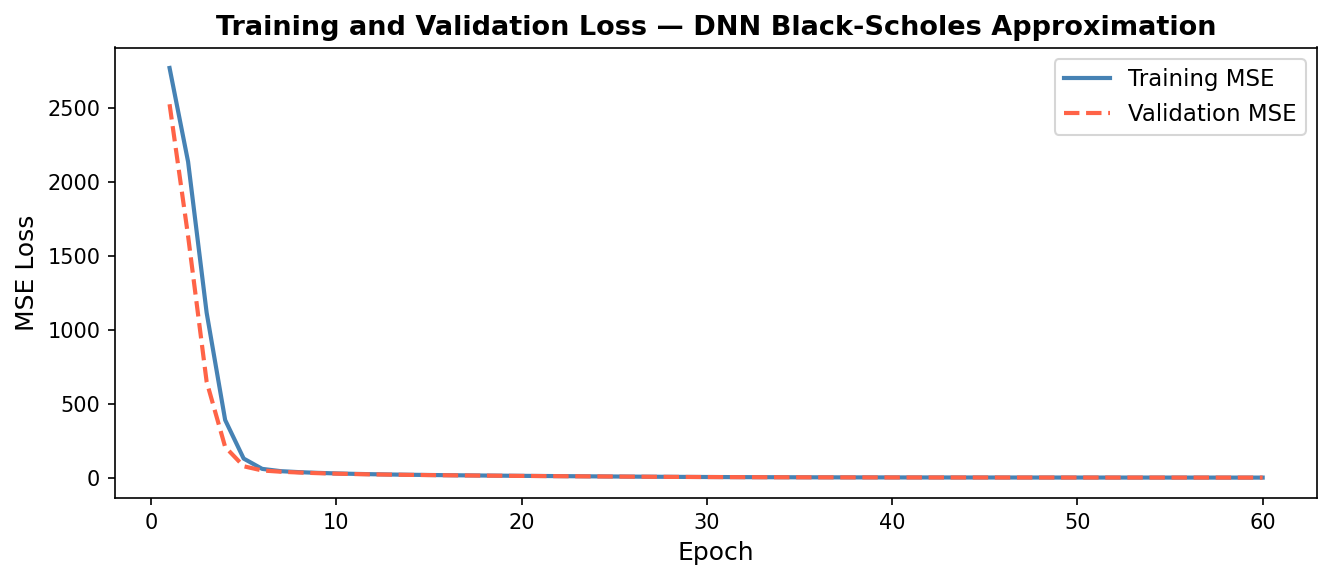
\includegraphics[width=0.75\textwidth]{figures/loss_curve.png}
    \caption{Training and validation MSE loss over 60 epochs for the Black-Scholes DNN surrogate ($B = 4096$, Adam, initial learning rate $10^{-3}$). Both curves are plotted on a linear scale with gridlines removed for readability.}
    \label{fig:dnn_bs_loss}
\end{figure}

The two curves sit almost on top of each other throughout, with no sign of the validation loss pulling away from the training loss, exactly what we would hope to see, and good evidence that the network is not overfitting to the training split (which would show up as a widening gap between the two curves). The scheduler fires a handful of times over the run, visible as small kinks in the rate of descent, and by epoch $60$ both curves have flattened out close to their final values.

\subsubsection{Out-of-Sample Accuracy}

Once training finishes, we evaluate the restored best-validation weights on the $20\%$ held-out test set, around $97{,}000$ option prices the network has never seen in any form. The headline numbers are
\begin{gather*}
\text{RMSE} = 1.4256, \quad \text{MAE} = 1.0769, \\
\text{Median Relative Error} = 3.0365\%, \quad \text{Max.\ Abs.\ Error} = 16.9364 .
\end{gather*}
Given that the simulated prices themselves range up into the hundreds, an RMSE of $1.43$ and a typical (median) relative error of about $3\%$ tell us the network has genuinely learned the shape of the pricing function, not merely memorised a lookup table.

One number, though, looks alarming at first glance: the \emph{mean} relative error comes out at $187{,}839.9048\%$. This is not a sign that the network is bad; it is an artefact of how relative error is defined, $|\hat C - C| / C$, when applied to options whose true price $C$ is extremely small. A deep out-of-the-money option, strike far above the current asset price for a call, or a very short time to maturity, can have a true Black-Scholes price of a few cents, or even a few thousandths of a unit, simply because it is almost certain to expire worthless. If the network's absolute error on such an option is, say, $0.05$, already an excellent prediction in absolute terms, but the true price is $0.0005$, the relative error on that single option alone is $10{,}000\%$. Average a few hundred such cases into a test set of $97{,}000$ options, and they alone are enough to drag the \emph{mean} up by orders of magnitude, even though the overwhelming majority of options are priced to within a few percent of their true value. The \emph{median} relative error of $3.0365\%$ is essentially immune to this (a handful of extreme outliers cannot move a median the way they move a mean) and is a far more honest summary of how the network performs on a typical option.

\subsubsection{Predicted vs.\ Actual Prices and the Residual Distribution}

Figure~\ref{fig:dnn_bs_eval} looks at the same test set from two complementary angles: the left-hand panel plots predicted price against true price for a random sample of $5{,}000$ test options alongside the line $y = x$ that a perfect model would lie on; the right-hand panel histograms the residuals $\hat C - C$ across the full test set.

\begin{figure}[htbp]
    \centering
    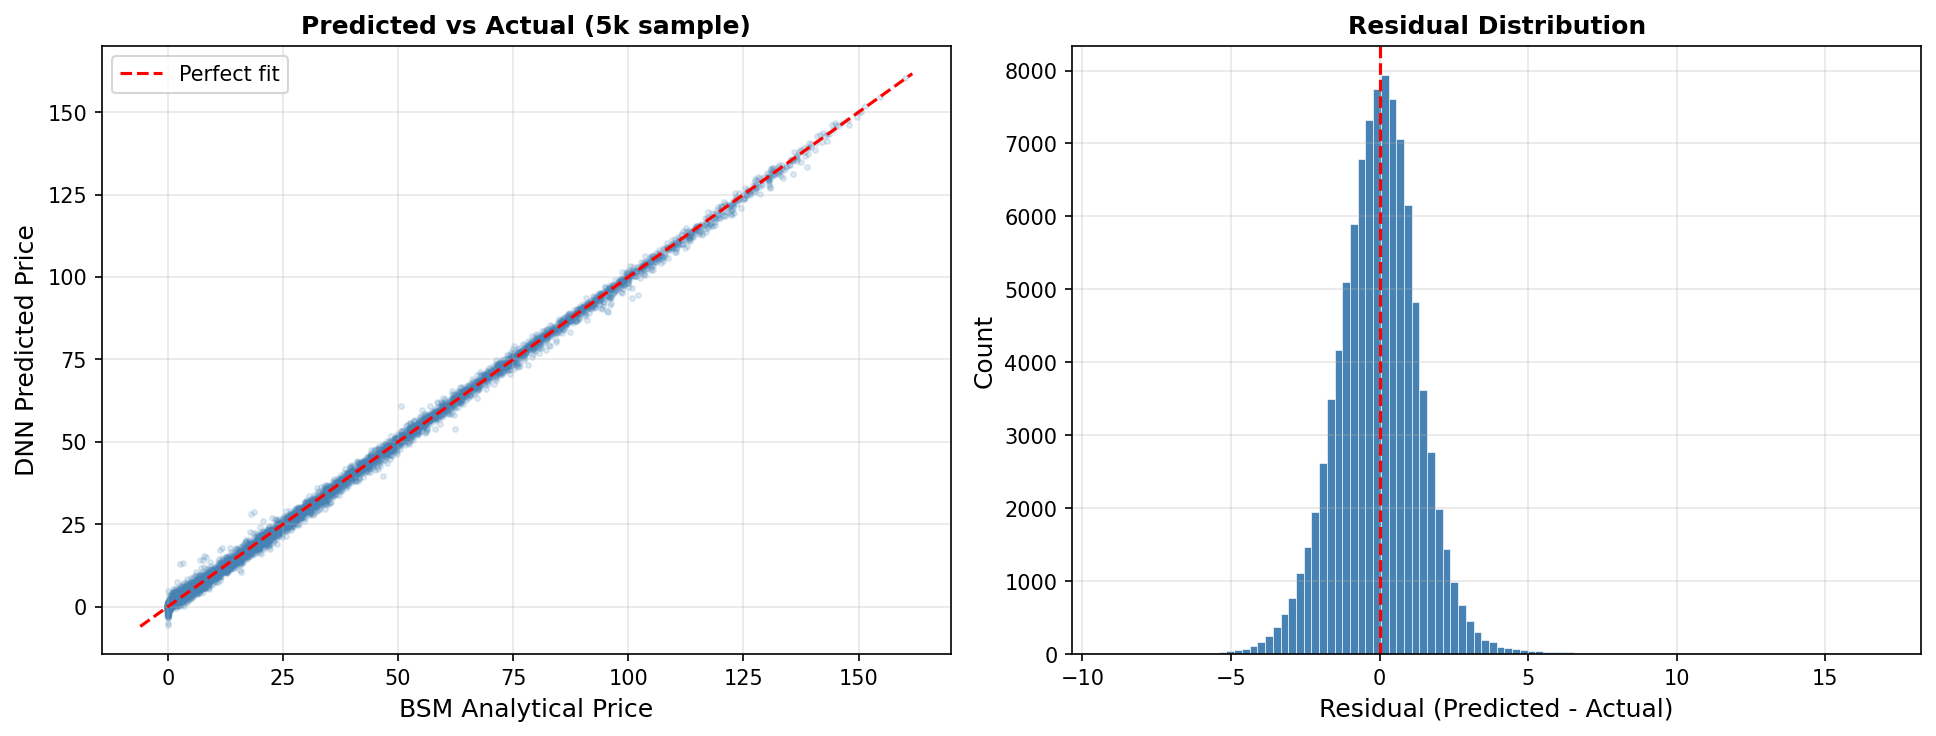
\includegraphics[width=0.95\textwidth]{figures/evaluation_plots.png}
    \caption{Out-of-sample evaluation of the Black-Scholes DNN surrogate on the held-out test set. \textit{Left:} predicted vs. true price for a random sample of 5,000 test options, with the dashed red line $y=x$ marking a perfect prediction. \textit{Right:} histogram of residuals $\hat C - C$ across the full test set, with the dashed red line marking zero error.}
    \label{fig:dnn_bs_eval}
\end{figure}

The scatter sits tightly along $y = x$ across the full range of prices, widening only mildly as the price grows, consistent with the small RMSE and median relative error reported above. The residual histogram is centred almost exactly on zero and roughly symmetric, telling us the network is not systematically over- or under-pricing on average; most of the mass sits within roughly $\pm 5$, with a longer tail reaching out towards $\pm 15$ corresponding to the harder, higher-priced end of the parameter space (typically the longer-dated, higher-volatility combinations). Neither plot shows any structural bias (no curvature in the scatter, no skew or multi-modality in the residuals), which is reassuring evidence that the $561$-parameter network has captured the global shape of the surface rather than fitting it well in some regions and badly in others in a way that would simply average out to a deceptively good RMSE.

\subsubsection{Speed Benchmark}

One of the main practical selling points of a trained surrogate is speed: once its $561$ weights are fixed, pricing an option is nothing more than two matrix multiplications and two ReLUs. Table~\ref{tab:dnn_bs_benchmark} compares, on a like-for-like, per-option basis, the cost of pricing via the closed-form Black-Scholes formula, via Monte Carlo simulation ($M = 10{,}000$ paths per option), and via a single batched forward pass through the trained network.

\begin{table}[htbp]
\centering
\caption{Per-option pricing cost (microseconds) for the Black-Scholes closed-form formula, Monte Carlo simulation ($M = 10{,}000$ paths), and the trained DNN surrogate (single batched forward pass, CPU). Speed-ups are quoted relative to the DNN.}
\label{tab:dnn_bs_benchmark}
\begin{tabular}{lcc}
\toprule
Method & Cost per option ($\mu$s) & Speed-up vs.\ DNN \\
\midrule
Closed-form (BSM) & 23.17 & $325\times$ \\
Monte Carlo ($M = 10^4$) & 135.84 & $1{,}907\times$ \\
DNN (batched forward pass) & 0.071 & --- \\
\bottomrule
\end{tabular}
\end{table}

The closed-form formula is already extremely fast, it is little more than a couple of calls to the normal CDF, and yet the trained network still beats it by a factor of roughly $325$, simply because pricing a whole batch of options is one vectorised operation rather than $N$ separate function calls. Against Monte Carlo, which has to simulate $10{,}000$ paths for every option it prices, the gap widens to nearly $1{,}900\times$. We have deliberately not visualised this comparison: the three methods span more than three orders of magnitude in cost per option, so a bar chart would either crush the DNN bar to invisibility on a linear axis or force a log axis of exactly the kind we have steered away from elsewhere in this section, the table above already makes the point more cleanly than a chart could. Where this speed advantage really bites in practice is in any task that prices the \emph{same} option repeatedly (calibrating a model to a whole surface of market-quoted prices, or computing Greeks by finite differences over a grid of bumped parameters), where the DNN's near-zero marginal cost compounds into a very real difference in wall-clock time.

\subsubsection{Pricing Surface}

Finally, Figure~\ref{fig:dnn_bs_surface} visualises the learned surface directly: the true Black-Scholes price, the DNN's prediction, and their absolute difference, all plotted as functions of $S$ and $K$ with the remaining parameters held fixed at representative values.

\begin{figure}[htbp]
    \centering
    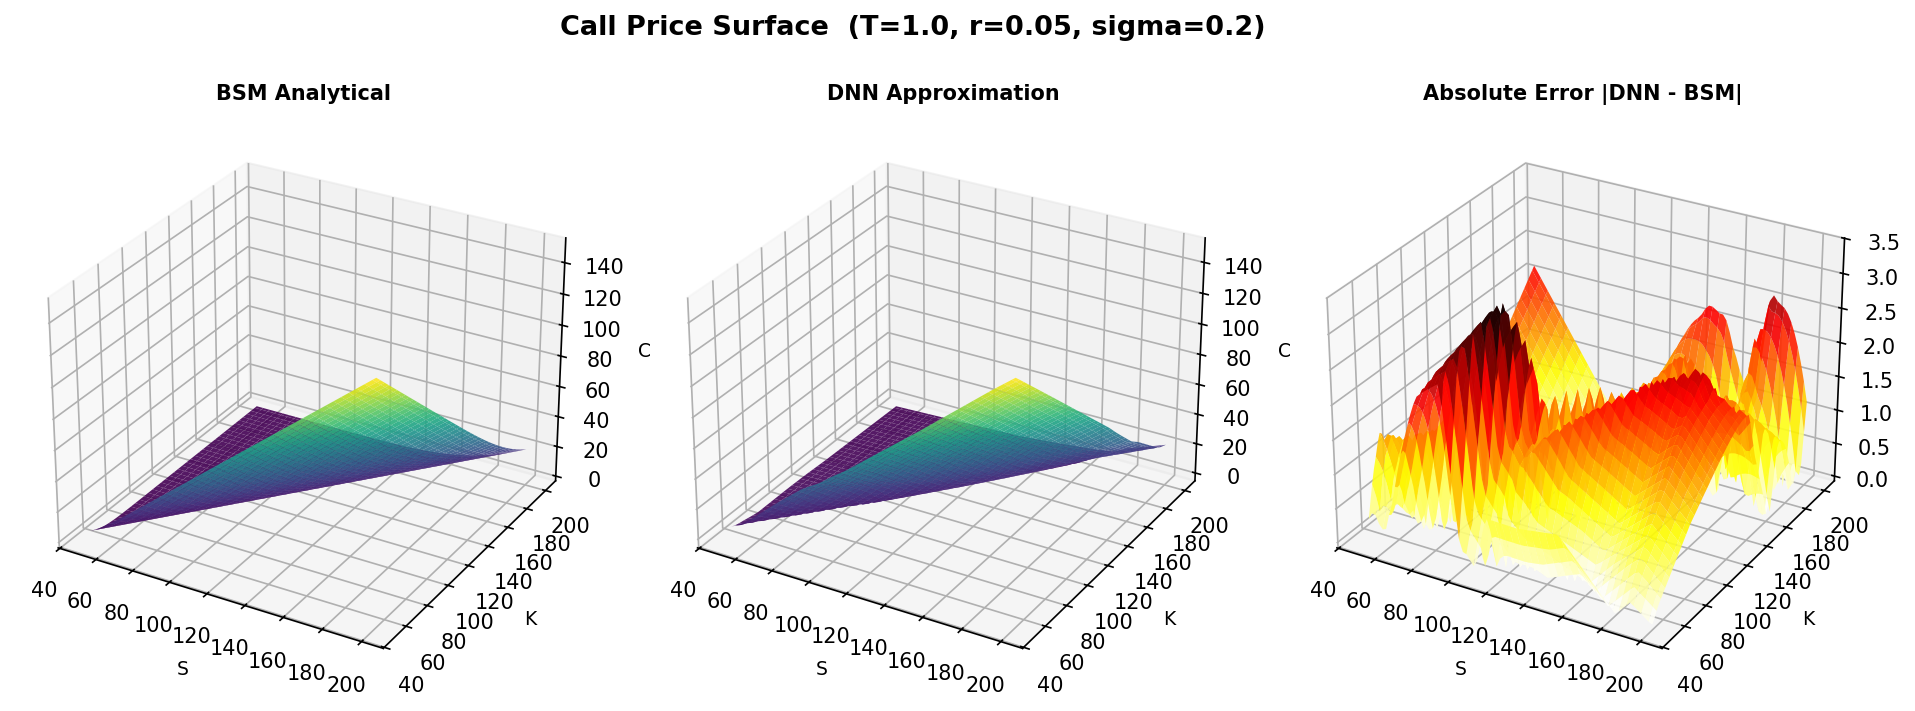
\includegraphics[width=0.95\textwidth]{figures/pricing_surface.png}
    \caption{Black-Scholes call price as a function of $(S, K)$: the true closed-form surface (left), the DNN's predicted surface (centre), and their absolute difference $|\hat C - C|$ (right), with $T$, $r$ and $\sigma$ held fixed at representative values.}
    \label{fig:dnn_bs_surface}
\end{figure}

The first two panels are visually almost indistinguishable; the network has clearly learned the surface's overall shape, including its convexity in $S$ and the way the price falls away as $K$ grows. The interesting panel is the third: the absolute error is close to zero across most of the $(S, K)$ plane, but rises noticeably in one corner (precisely the deep out-of-the-money region where $S \ll K$, so the call is far from ever being exercised) and, to a lesser extent, for short-dated, low-volatility combinations where the true price is similarly close to zero. This is exactly the same region responsible for the inflated mean relative error discussed earlier: the \emph{absolute} error there is actually one of the smallest on the whole surface in raw terms, but because the true price in that corner is itself only a few cents, that small absolute error corresponds to an enormous relative one. The surface plot and the mean-relative-error anomaly are, in other words, two views of the same fact: the network's worst \emph{relative} performance occurs exactly where its \emph{absolute} performance is at its best, simply because that is also where the target itself is smallest. Away from that corner, the surface is well-captured throughout, which is, ultimately, the more important takeaway.

\FloatBarrier
\subsection{Monte Carlo Simulation under the Heston Model}

Unlike the simple Black-Scholes model, the Heston stochastic volatility model assumes the variance of the underlying asset follows a mean-reverting square root process. As an alternative to evaluating semi-closed formulas or constructing a Finite Difference grid, we can adapt our Monte Carlo framework to price options under this stochastic volatility.

Under the risk-neutral measure, the price process of the risky asset $S_t$ and its variance $V_t$ satisfy the following system of Stochastic Differential Equations (SDEs) for $0 \le t \le T$:

\begin{equation}
dS_t = r S_t dt + \sqrt{V_t} S_t dW_t
\end{equation}
\begin{equation}
dV_t = \kappa(\theta - V_t) dt + \omega \sqrt{V_t} dW_t^1
\end{equation}

where $r$ is the constant risk-free interest rate with continuous compounding. The parameters $\kappa, \theta$, and $\omega$ are positive constants satisfying $2\kappa\theta \ge \omega^2$, representing the mean reversion speed, mean reversion level, and volatility of $V_t$, respectively. $W_t$ and $W_t^1$ are standard Brownian motions with correlation $\rho \in (-1, 1)$. 

To simulate this system computationally, we can write $W_t^1$ equivalently as a combination of two independent standard Brownian motions, $W_t$ and $\tilde{W}_t$:

\begin{equation}
W_t^1 = \rho W_t + \sqrt{1 - \rho^2} \tilde{W}_t
\end{equation} 

To generate sample paths of $S$ and $V$ over the interval $[0, T]$, we divide the interval into $n$ equally spaced subintervals with grid points $t_i = i h$ for $i=0, 1, \dots, n$, where the step size is $h = T/n$. At each step, we generate $2n$ independent standard normal variables $Z_i$ and $\tilde{Z}_i$. The discrete Euler-Maruyama approximations are given by:

\begin{equation}
S_{t_i} = S_{t_{i-1}} + r S_{t_{i-1}} h + \sqrt{V_{t_{i-1}}^+} S_{t_{i-1}} \sqrt{h} Z_i
\end{equation}

\begin{equation}
V_{t_i} = V_{t_{i-1}} + \kappa(\theta - V_{t_{i-1}}^+) h + \omega \sqrt{V_{t_{i-1}}^+} \sqrt{h} (\rho Z_i + \sqrt{1 - \rho^2} \tilde{Z}_i)
\end{equation}

with the initial conditions $S_{t_0} = S_0$ and $V_{t_0} = V_0$. 

Note that although in theory $V_t > 0$ for all $t$, in numerical computation, it is possible to have $V_t \le 0$. Because $\sqrt{V_t}$ is not well-defined in that case, we apply a truncation scheme by replacing $V_{t_{i-1}}$ with $V_{t_{i-1}}^+ = \max(V_{t_{i-1}}, 0)$.

Given time $t=0$, the European call price is given by the expectation:

\begin{equation}
C(0, S, V) = E[e^{-rT}(S_T - K)^+]
\end{equation} 

To compute this expectation using the simulation method, we generate sample paths of $S$ and $V$, evaluate the terminal payoff $(S_T - K)^+$, and repeat this $M$ times to get the average. Finally, we multiply by the discount factor $e^{-rT}$ to obtain the estimated option price $\hat{C}$:

\begin{equation}
\hat{C}(0, S_0, V_0) = e^{-rT} \frac{1}{M} \sum_{m=1}^{M} \left( S_{t_n}^{(m)} - K \right)^+
\end{equation}

(where $S_{t_n}^{(m)}$ represents the terminal stock price $S_T$ of the $m$-th simulated path).

\subsubsection{Discretisation Convergence: How Many Time Steps Are Enough?}

One aspect of the Heston Monte Carlo that has no direct parallel in the Black-Scholes case is the role of the number of time steps $n$. In the Black-Scholes framework, we exploited the exact closed-form solution for $S_T$ and jumped directly to the terminal price in a single step. Under the Heston model, no such shortcut exists; the Euler-Maruyama scheme is an approximation, and the discretisation step size $h = T/n$ introduces a bias that depends on $n$. This gives us an extra dimension to investigate.

Figure~\ref{fig:heston_timestep} shows the MC price against $n$ for fixed $M = 2 \times 10^5$ paths, with the semi-analytic Heston price as the reference.

\begin{figure}[htbp]
    \centering
    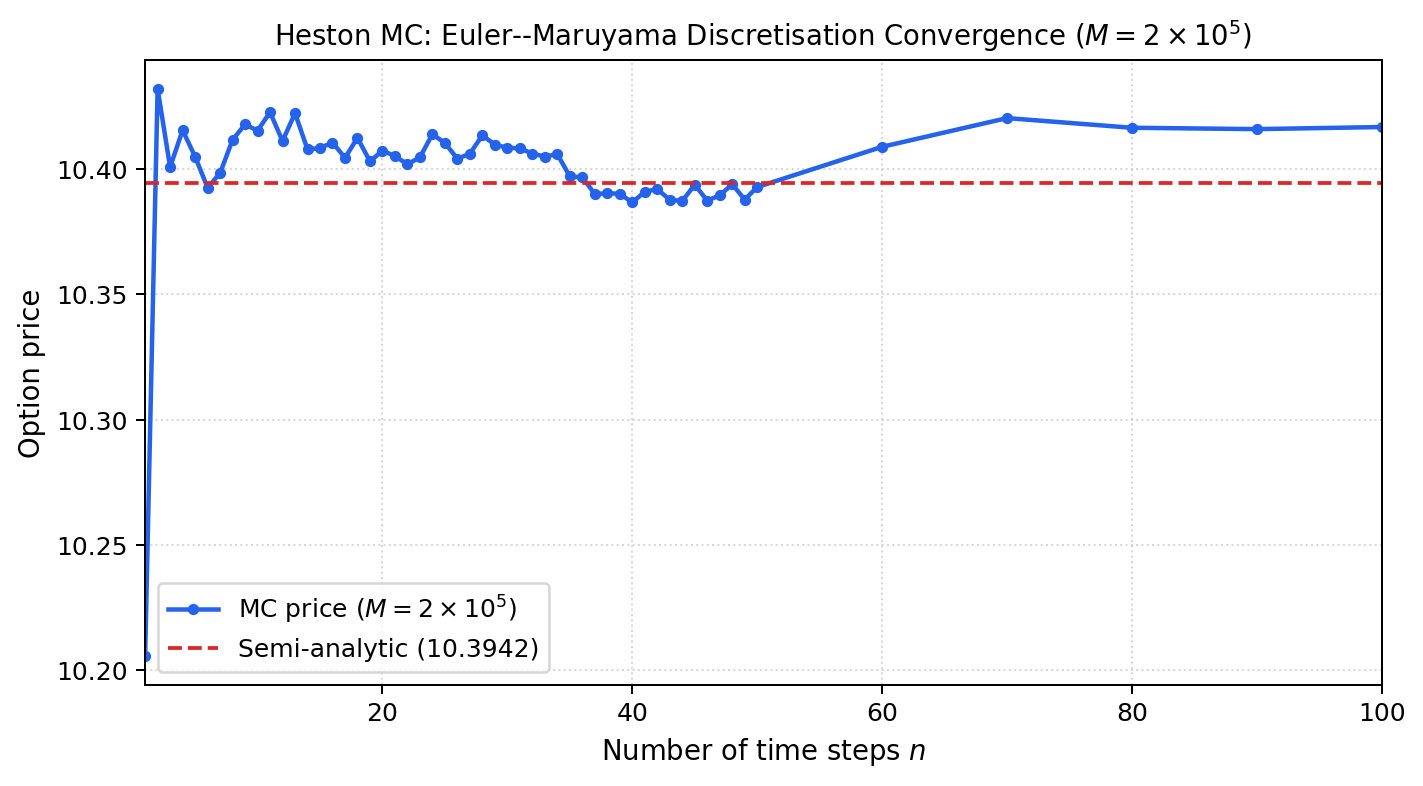
\includegraphics[width=0.9\textwidth]{figures/heston_timestep_convergence.png}
    \caption{Heston MC price as a function of the number of Euler--Maruyama time steps $n$, with $M = 2\times10^5$ paths fixed. Parameters: $S_0 = K = 100$, $T=1$, $r=0.05$, $\kappa=2$, $\theta=0.04$, $\omega=0.3$, $\rho=-0.7$, $V_0=0.04$. The dashed line is the semi-analytic Heston price (10.3942).}
    \label{fig:heston_timestep}
\end{figure}

At $n=1$, the estimate is clearly biased; a single large step cannot capture the mean-reverting behaviour of $V_t$ over the interval $[0,T]$, resulting in an underestimate of around 0.19. By $n \approx 5$, the price has essentially converged to the semi-analytic reference. The residual fluctuation at larger $n$ is not discretisation error but rather MC sampling noise: since $M$ is held fixed, the noise floor stays constant regardless of how finely we discretise time.

The practical implication is that the choice of $n$ is not critical, once it is past a moderate threshold, increasing it further only adds computational cost without improving accuracy. For these parameters, $n = 50$ is more than sufficient.

\FloatBarrier

\subsubsection{Parameter Sensitivity: Effect of Correlation $\rho$}

The correlation parameter $\rho$ has no analogue in the Black-Scholes model; it is a purely Heston quantity that captures the relationship between movements in the asset price and movements in its variance. In equity markets, $\rho$ is typically negative: when the stock price falls, volatility tends to spike, a stylised fact known as the \textit{leverage effect} \cite{black1976}.

The intuition becomes clearer when thinking about different market participants. For a high-growth, high-valuation stock, a price drop tends to trigger traders to exit and take profits, amplifying the sell-off and driving volatility higher, this corresponds to $\rho < 0$. By contrast, for a stable, cash-generative business (a ``cash cow''), long-term holders tend not to react to short-term price movements, so a price decline does not trigger a corresponding volatility spike, this behaviour is closer to $\rho > 0$.

The impact on European call option pricing follows directly from this mechanism. When $\rho < 0$, a falling stock price is accompanied by rising volatility: if the option goes out-of-the-money, the surge in volatility gives it a greater chance of recovering back into the money before expiry. This makes the call more valuable. When $\rho > 0$, a falling price is accompanied by falling volatility, so an out-of-the-money option is unlikely to recover. The call is therefore cheaper.

Figure~\ref{fig:heston_rho} confirms this: the MC price decreases monotonically as $\rho$ increases from $-0.98$ to $+0.98$. It is worth noting that the behaviour at the extremes ($\rho \to \pm 1$) is a degenerate mathematical limit of the model; perfect correlation between the two Brownian motions is not an economically meaningful regime, and the price behaviour there is driven by the mean-reversion structure built into the model rather than real market dynamics.

\begin{figure}[htbp]
    \centering
    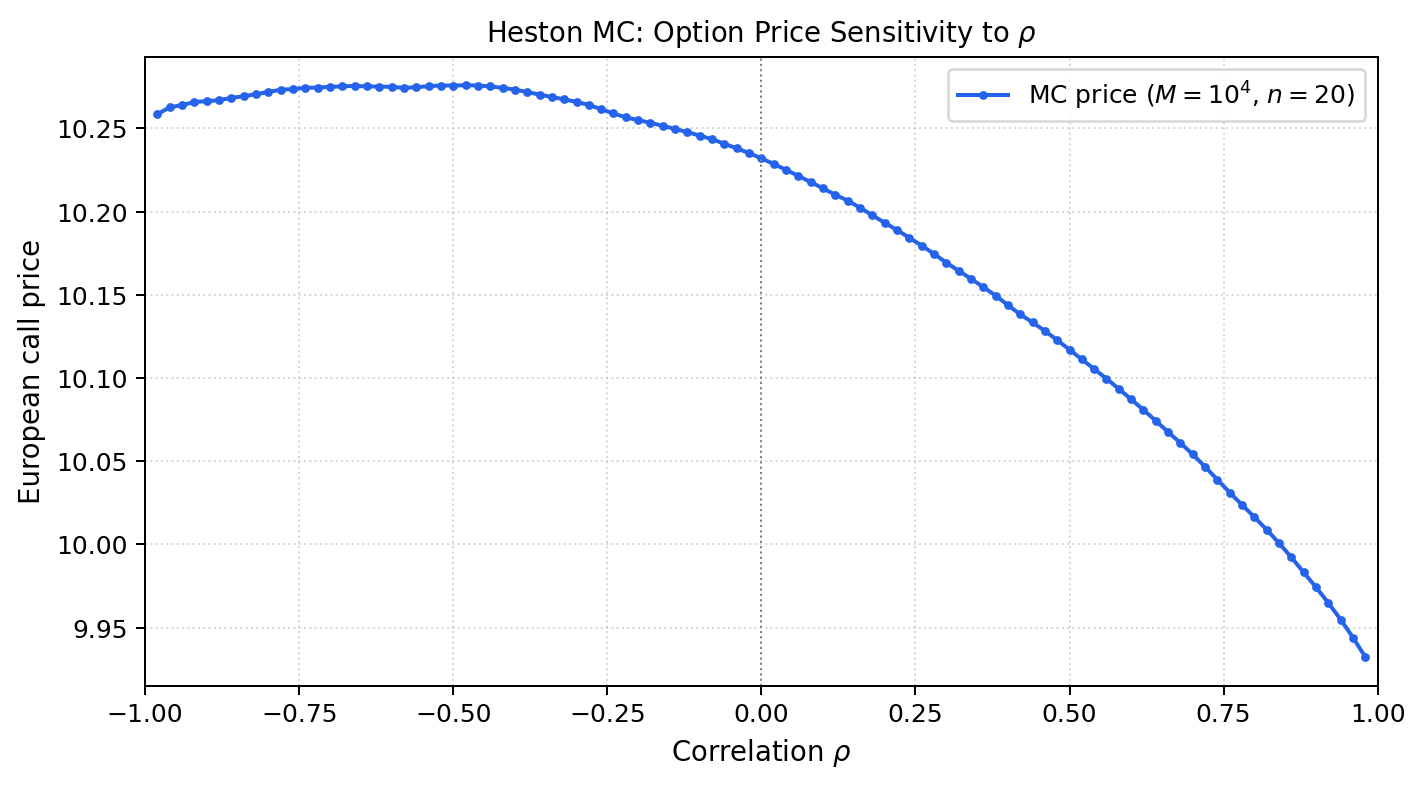
\includegraphics[width=0.9\textwidth]{figures/heston_rho_sensitivity.png}
    \caption{European ATM call price as a function of the correlation parameter $\rho$, computed via Monte Carlo with $M=10^4$ paths and $n=20$ time steps at each of 99 equally spaced values from $-0.98$ to $+0.98$. Other parameters: $S_0=K=100$, $T=1$, $r=0.05$, $\kappa=2$, $\theta=0.04$, $\omega=0.3$, $V_0=0.04$.}
    \label{fig:heston_rho}
\end{figure}

\FloatBarrier

\subsubsection{Parameter Sensitivity: Effect of Vol of Vol $\omega$}

The parameter $\omega$ controls the volatility of the variance process, intuitively, how ``uncontrolled'' the variance becomes. We set $\rho = 0$ to isolate the pure $\omega$ effect, and plot only up to the Feller boundary $\omega^* = \sqrt{2\kappa\theta} = 0.8$; beyond this point the variance process can reach zero, the truncation scheme activates, and results become unreliable.

\begin{figure}[htbp]
    \centering
    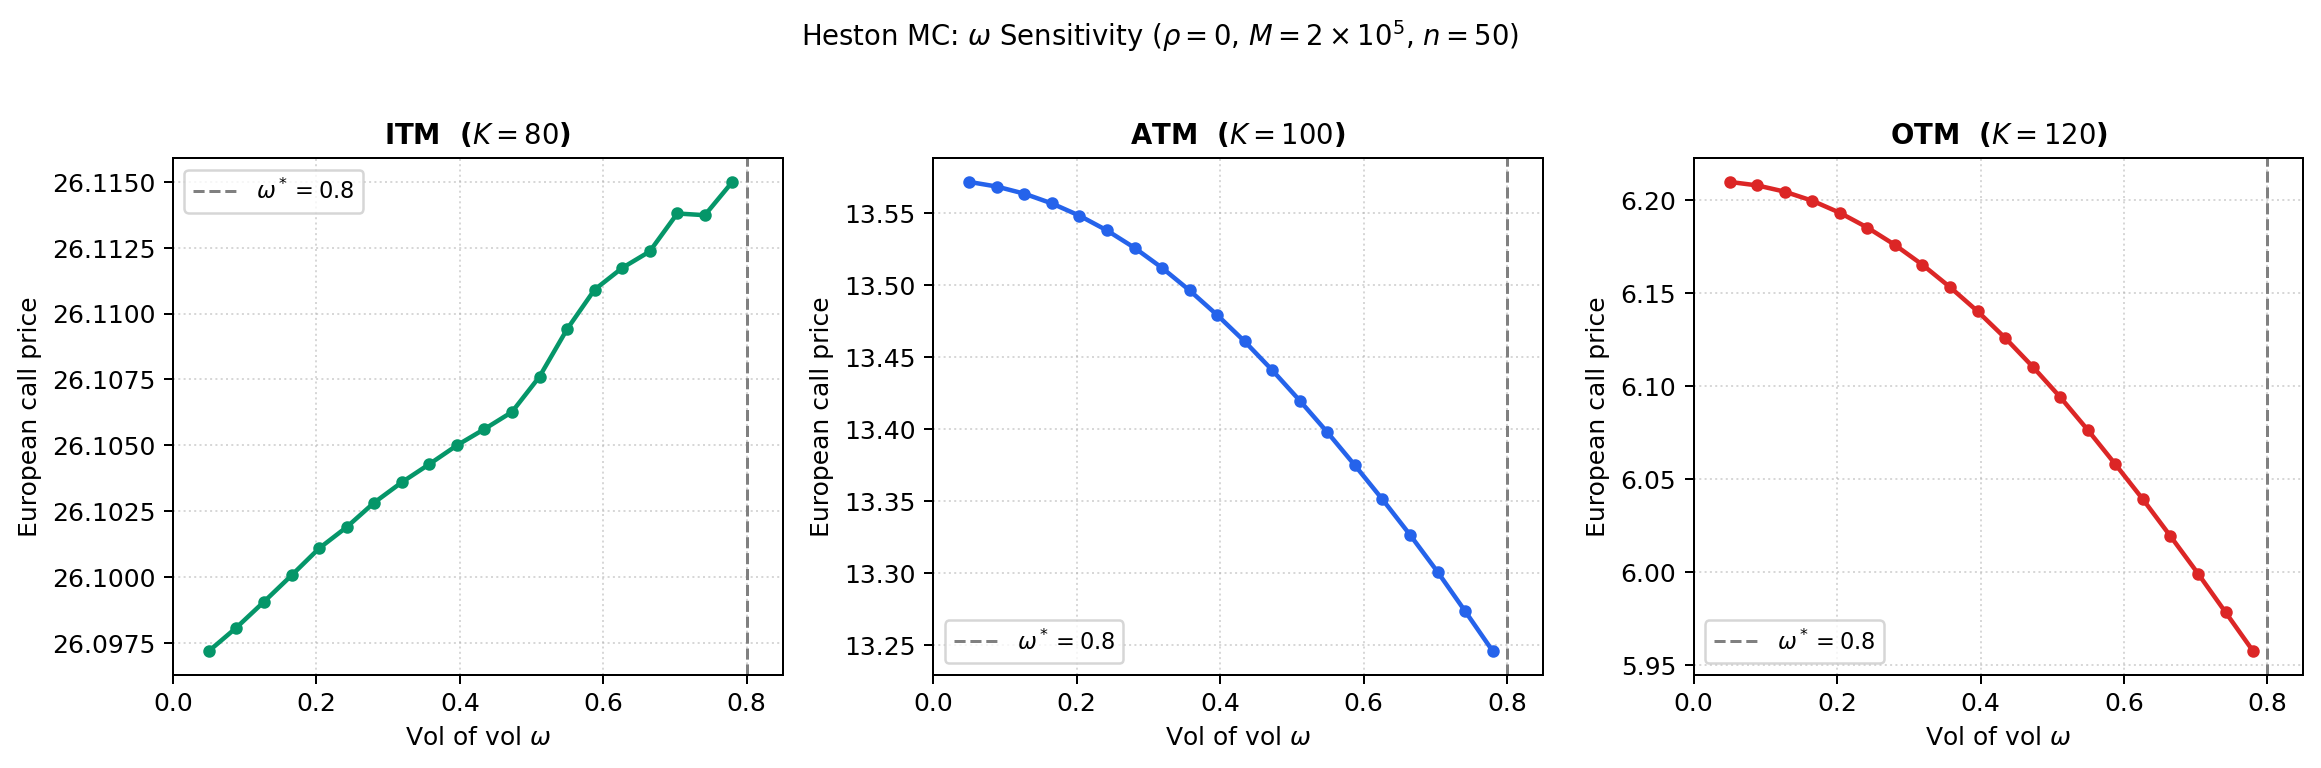
\includegraphics[width=\textwidth]{figures/heston_omega_sensitivity.png}
    \caption{European call price as a function of $\omega$ for ITM ($K=80$), ATM ($K=100$), and OTM ($K=120$), computed via MC with $M=2\times10^5$ paths and $n=50$ time steps. Parameters: $S_0=100$, $T=1$, $r=0.05$, $\kappa=4$, $\theta=0.08$, $V_0=0.08$, $\rho=0$. The dashed vertical line marks the Feller boundary $\omega^*=0.8$.}
    \label{fig:heston_omega}
\end{figure}

The three panels tell different stories. The ITM panel ($K=80$) is essentially flat: the price barely changes from $26.10$ to $26.12$ across the full $\omega$ range. The ATM panel ($K=100$) shows a clear monotonic decrease of around $0.33$. The OTM panel ($K=120$) also decreases, but less steeply (around $0.25$).

The reason comes down to the curvature of the Black-Scholes price in $\sigma$. With $\rho = 0$, the Heston price can be written as an expectation of Black-Scholes prices over the distribution of the realised average volatility $\bar{\sigma} = \sqrt{\frac{1}{T}\int_0^T V_t \, dt}$:
\begin{equation}
    C_{\text{Heston}} = \mathbb{E}\left[ C_{\text{BS}}\!\left(\bar{\sigma}\right) \right]
\end{equation}
Increasing $\omega$ spreads the distribution of $\bar{\sigma}$ without changing its mean (since variance mean-reverts to $\theta$). Whether this raises or lowers $C_{\text{Heston}}$ depends on whether $C_{\text{BS}}(\sigma)$ is convex or concave in $\sigma$ at that moneyness. By Jensen's inequality:
\begin{equation}
    C_{\text{BS}} \text{ concave in } \sigma \implies \mathbb{E}\left[C_{\text{BS}}(\bar{\sigma})\right] \leq C_{\text{BS}}\!\left(\mathbb{E}[\bar{\sigma}]\right)
\end{equation}
The second derivative of the Black-Scholes price with respect to $\sigma$ is:
\begin{equation}
    \frac{\partial^2 C_{\text{BS}}}{\partial \sigma^2} = S_0 \sqrt{T} \, \phi(d_1) \, \frac{d_1 d_2}{\sigma}
\end{equation}
For an ATM call, $d_1 \approx \tfrac{1}{2}\sigma\sqrt{T} > 0$ and $d_2 \approx -\tfrac{1}{2}\sigma\sqrt{T} < 0$, so $d_1 d_2 < 0$ and the price is concave in $\sigma$; more spread in $\bar{\sigma}$ lowers the price. For an OTM call, both $d_1$ and $d_2$ are negative, so $d_1 d_2 > 0$ and the price is convex in $\sigma$; more spread should raise the price. However, at $K=120$ the convexity effect is modest and is partially offset by the same concavity near mid-range $\sigma$, resulting in a small net decrease. For the deep ITM case ($K=80$), both $d_1$ and $d_2$ are large and positive, the option value is dominated by its intrinsic value of $\approx 25$, and the time-value component contributing sensitivity to $\omega$ is negligible, hence the flat response.

\FloatBarrier

\subsubsection{Numerical Validation Against the Semi-Analytic Price}

To verify the Heston Monte Carlo estimator, we compare it against the semi-analytic Heston formula across four moneyness regimes, using $\kappa=2$, $\theta=0.04$, $\omega=0.3$, $\rho=-0.7$, $V_0=0.04$, $r=0.05$, $T=1$, and $M=10^4$ paths with $n=50$ steps.

\begin{table}[htbp]
\centering
\caption{Heston Monte Carlo vs.\ semi-analytic price for $M=10^4$ paths, $n=50$, $r=0.05$, $T=1$.}
\label{tab:heston_validation}
\begin{tabular}{lcccccccc}
\toprule
Scenario & $S_0$ & $K$ & SA Price & MC Price & 95\% CI & SE & Abs Err & \% Err \\
\midrule
Deep ITM    & 120 & 100 & 26.7305 & 26.6052 & $[26.22,\ 26.99]$ & 0.1963 & 0.1253 & 0.47 \\
ATM         & 100 & 100 & 10.3942 & 10.2801 & $[10.04,\ 10.52]$ & 0.1222 & 0.1141 & 1.10 \\
Slight OTM  &  95 & 100 &  7.1712 &  7.0825 & $[\ 6.89,\ \ 7.28]$ & 0.1001 & 0.0887 & 1.24 \\
Deep OTM    &  80 & 100 &  1.1246 &  1.1129 & $[\ 1.04,\ \ 1.18]$ & 0.0352 & 0.0116 & 1.03 \\
\bottomrule
\end{tabular}
\end{table}

The percentage errors stay below 1.3\% across all cases. The deep OTM case has the smallest SE (0.035) and absolute error, since most paths expire worthless and payoff variance is low. The pattern mirrors the Black-Scholes validation in Section~\ref{tab:mc_validation}: the high-volatility, high-uncertainty cases demand more paths for the same precision.

\FloatBarrier

\subsubsection{Heston vs.\ Black-Scholes: When Do They Diverge?}

The Heston model reduces to Black-Scholes when $\kappa \to \infty$ and $\theta = V_0$; the variance is pinned at $V_0$ and never moves, so both models price identically with $\sigma = \sqrt{V_0}$. In practice, $\kappa$ is finite and $\theta \neq V_0$, meaning the variance has a long-run level it is drifting towards. This is the key structural difference that Black-Scholes cannot capture.

Figure~\ref{fig:heston_vs_bs} plots $|C_{\text{Heston}} - C_{\text{BS}}|$ over the $(\kappa, \theta)$ plane, with $V_0 = 0.04$ fixed so the Black-Scholes price uses $\sigma = \sqrt{V_0} = 0.2$. Parameters $\omega = 0.3$ and $\rho = -0.5$ are held constant. The dotted grey curve marks the Feller boundary $2\kappa\theta = \omega^2$; the region below it is masked. The dashed blue line marks $\theta = V_0 = 0.04$, this is where the variance starts exactly at its long-run mean, so there is no systematic drift and the two models are closest to each other.

\begin{figure}[htbp]
    \centering
    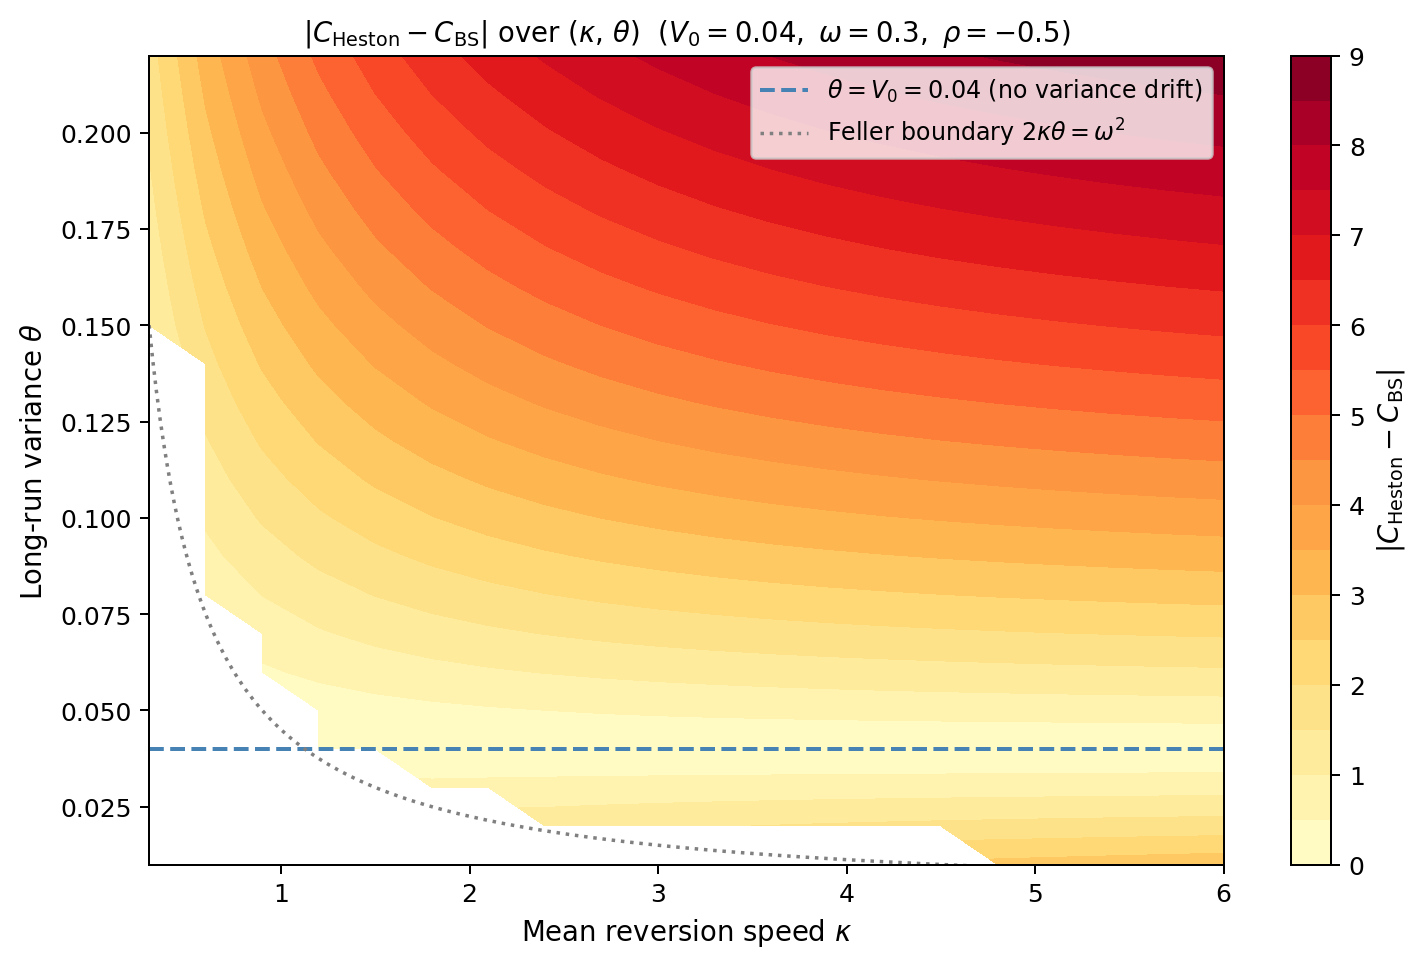
\includegraphics[width=0.9\textwidth]{figures/heston_vs_bs_heatmap.png}
    \caption{Absolute price difference $|C_{\text{Heston}} - C_{\text{BS}}|$ over the $(\kappa,\theta)$ plane for an ATM call with $S_0=K=100$, $T=1$, $r=0.05$, $V_0=0.04$, $\omega=0.3$, $\rho=-0.5$. The Black-Scholes price uses $\sigma=\sqrt{V_0}=0.2$. The dashed line at $\theta=V_0=0.04$ marks where variance starts at its long-run mean (no drift); the dotted curve is the Feller boundary $2\kappa\theta=\omega^2$.}
    \label{fig:heston_vs_bs}
\end{figure}

The heatmap shows two clear drivers of divergence. The dashed line at $\theta = V_0$ is where the difference is smallest for large $\kappa$; variance has no drift, so for fast mean reversion the models agree closely. Move away from this line in either direction (higher or lower $\theta$) and the difference grows, because Heston is now pricing in a variance drift that Black-Scholes ignores entirely. The second driver is $\kappa$: slow mean reversion (left side of the plot) dramatically amplifies the divergence. When $\kappa$ is small, the variance has more time over $[0,T]$ to drift toward $\theta$, so the gap between the effective volatility in Heston and the fixed $\sigma$ in Black-Scholes widens. In the extreme corner of slow $\kappa$ and high $\theta$, the difference reaches nearly 9; a Black-Scholes model calibrated to current volatility would severely underprice the option in that regime.

\FloatBarrier
\subsection{Deep Neural Network Pricing under the Heston Model}

Having built and validated the whole pipeline in Section~\ref{sec:dnn_bs}, extending it to Heston turns out to be mostly a matter of \emph{scale} rather than a fresh design exercise; the data-generation, normalisation, architecture and training code all carry over with only the natural adjustments that come from moving to a nine-dimensional input space.

\subsubsection{Scaling Up: Data, Normalisation and Architecture}

The Heston price depends on nine inputs rather than five: the original four $(S, K, T, r)$, plus the five parameters governing the variance process, $(V_0, \kappa, \theta, \omega, \rho)$, so $d$ jumps from $5$ to $9$. As in Chapter 1, we draw $500{,}000$ parameter combinations by uniform random sampling, now over nine ranges ($V_0 \in [0.01, 0.50]$, $\kappa \in [0.1, 5.0]$, $\theta \in [0.01, 0.50]$, $\omega \in [0.05, 1.0]$, $\rho \in [-0.75, 0.75]$, with $S, K, T, r$ unchanged from Chapter 1), and label each one with the Heston semi-analytic price obtained by numerically integrating the model's characteristic function \cite{heston1993}, the same noise-free-label philosophy as before, now with a considerably more expensive labelling step (a numerical integration per price, rather than a couple of calls to the normal CDF, which is part of why this dataset took noticeably longer to build). Rows whose price comes out below $10^{-6}$ (degenerate, essentially worthless combinations from extreme-OTM or near-zero-maturity draws) are dropped before training.

We fit a brand-new \texttt{StandardScaler} to these nine inputs rather than reusing the Black-Scholes one: the two sets of variables live on genuinely different scales (compare $\kappa \in [0.1, 5.0]$ with $\rho \in [-0.75, 0.75]$, or $S \in [50, 200]$ with $V_0 \in [0.01, 0.50]$), and reusing statistics fitted on a different set of variables would simply reintroduce the very scale-mismatch problem normalisation exists to solve.

The network itself is the same \texttt{OptionPricingDNN} class with \texttt{input\_dim=9} and two hidden layers, but each layer is widened from $20$ to $40$ neurons. A nine-dimensional input is a substantially richer object to map into a price than a five-dimensional one, there are simply more interactions for the network to represent (how does the effect of $\rho$ on the price change as $\kappa$ varies? as $V_0$ varies?), and a wider hidden layer gives it the room to do so. Plugging $d = 9, n = 40$ into the parameter-count formula from Section~\ref{sec:dnn_bs},
\[
P(9, 40) = 40^2 + (9 + 3)\cdot 40 + 1 = 1600 + 480 + 1 = 2{,}081,
\]
gives a network with $2{,}081$ trainable parameters, about $3.7$ times the size of the Black-Scholes network, which seems a perfectly reasonable price to pay for handling nearly double the input dimension while (as the results below confirm) reaching comparable accuracy on a considerably harder surface. Training itself is identical: the same loss (MSE), the same optimiser (Adam \cite{kingma2015}, learning rate $10^{-3}$, with the same plateau scheduler), the same $60$ epochs and batch size of $4{,}096$. The training loop in Chapter 1 was written generically enough that retargeting it at this new model required no changes whatsoever.

\subsubsection{Training Behaviour and Out-of-Sample Accuracy}

Figure~\ref{fig:dnn_heston_loss} shows the training and validation loss curves, plotted in the same linear, gridless style as Figure~\ref{fig:dnn_bs_loss} for direct comparison.

\begin{figure}[htbp]
    \centering
    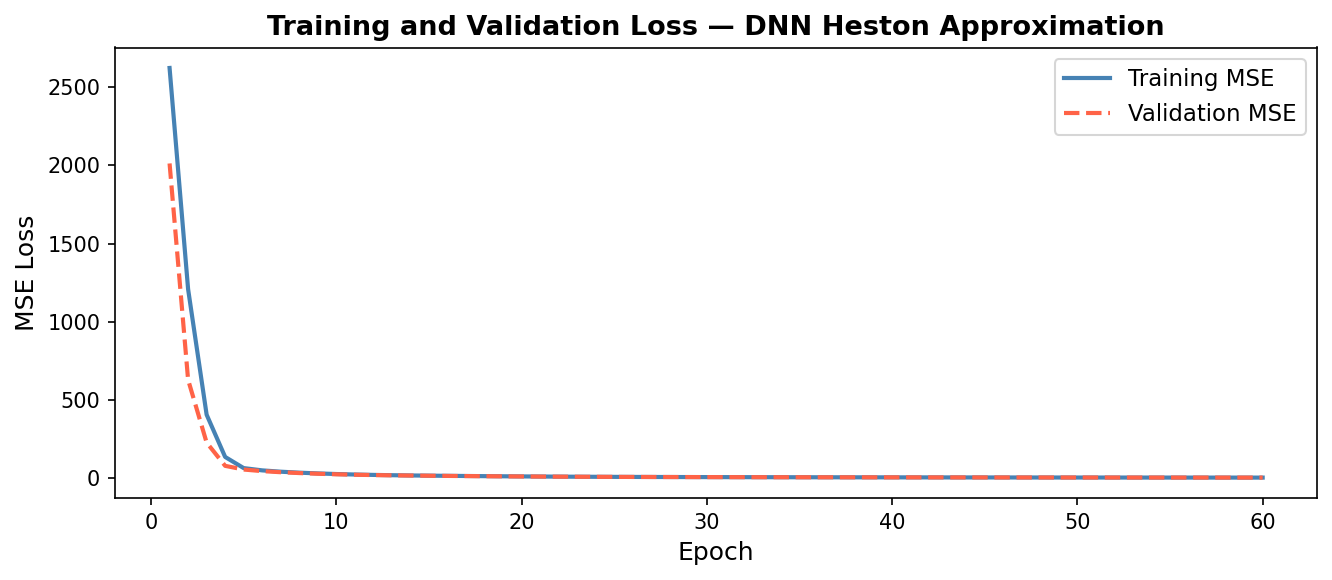
\includegraphics[width=0.75\textwidth]{figures/heston_loss_curve.png}
    \caption{Training and validation MSE loss over 60 epochs for the Heston DNN surrogate (input dimension 9, two hidden layers of 40 neurons, $B = 4096$, Adam, initial learning rate $10^{-3}$).}
    \label{fig:dnn_heston_loss}
\end{figure}

The pattern mirrors Chapter 1 closely: training and validation loss fall together with no widening gap between them, and both flatten out by the end of the $60$ epochs. On the held-out test set (around $99{,}000$ options), the network achieves
\begin{gather*}
\text{RMSE} = 1.6129, \quad \text{MAE} = 1.0803, \\
\text{Median Relative Error} = 2.7597\%, \quad \text{Max.\ Abs.\ Error} = 33.7062 .
\end{gather*}
These figures sit close to, if very slightly weaker than, the Black-Scholes results (RMSE $1.43$, median relative error $3.04\%$), which we read as a genuinely encouraging outcome: despite having to learn a surface that is nearly twice as wide in input dimension and considerably more intricate (the Heston price now depends on the entire path of a correlated stochastic-variance process, not on a single constant $\sigma$), a network with roughly $3.7$ times as many parameters reaches essentially the same level of accuracy. The same deep-OTM pathology diagnosed in Chapter~1 reappears here too; the mean relative error again comes out enormous, of order $10^4\%$ ($19{,}423.32\%$), for exactly the same reason: a small number of near-worthless test options whose true prices sit close to zero. As before, though, the median relative error of $2.7597\%$, if anything marginally \emph{better} than the Black-Scholes figure, is the number that actually describes how the network performs on a typical option.

Figure~\ref{fig:dnn_heston_eval} repeats the predicted-vs-actual and residual analysis from Chapter 1.

\begin{figure}[htbp]
    \centering
    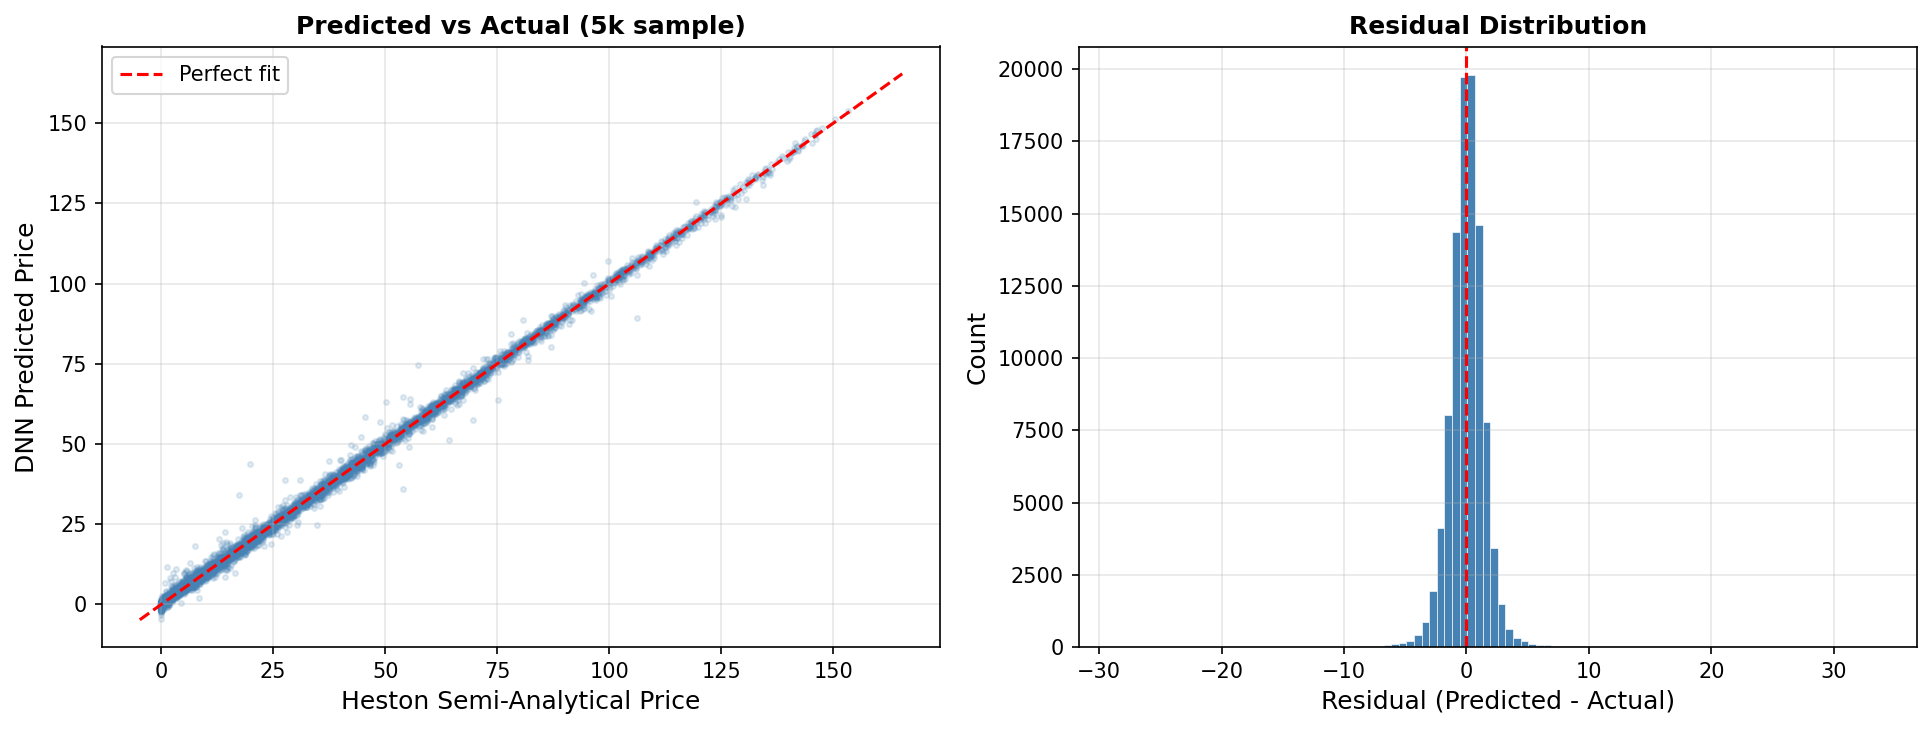
\includegraphics[width=0.95\textwidth]{figures/heston_evaluation_plots.png}
    \caption{Out-of-sample evaluation of the Heston DNN surrogate. \textit{Left:} predicted vs. true price for a random sample of 5,000 test options, with the dashed red line $y = x$ marking a perfect prediction. \textit{Right:} histogram of residuals $\hat C - C$, with the dashed red line marking zero error.}
    \label{fig:dnn_heston_eval}
\end{figure}

The scatter again clusters tightly along $y = x$, and the residuals are again centred close to zero and roughly symmetric, with no systematic bias visible in either panel. The one clear difference from Chapter 1 is the spread: the Heston residuals range out to roughly $\pm 30$, against roughly $\pm 15$ for Black-Scholes, exactly consistent with the larger maximum absolute error reported above ($33.71$ vs. $16.94$). This wider spread is the natural fingerprint of a harder, higher-dimensional surface: there are simply more ways for nine correlated inputs to combine into an unusual, hard-to-fit price than there are for five.

\subsubsection{Speed Benchmark}

The speed comparison is, if anything, even more striking here than in Chapter 1, precisely because both "ground truth" methods become substantially more expensive once volatility is allowed to be stochastic: the semi-analytic price needs a numerical integration of the characteristic function for every single option, and Monte Carlo now has to simulate the joint $(S_t, V_t)$ system step by step (we use the Euler--Maruyama scheme with full truncation, $100$ time steps and $10{,}000$ paths per option) rather than sampling the terminal price directly in one shot. Table~\ref{tab:dnn_heston_benchmark} reports the same like-for-like, per-option comparison as before.

\begin{table}[htbp]
\centering
\caption{Per-option pricing cost (microseconds) for the Heston semi-analytic price, Monte Carlo simulation ($N_{\text{steps}} = 100$, $M = 10{,}000$ paths), and the trained DNN surrogate. Speed-ups are quoted relative to the DNN.}
\label{tab:dnn_heston_benchmark}
\begin{tabular}{lcc}
\toprule
Method & Cost per option ($\mu$s) & Speed-up vs.\ DNN \\
\midrule
Semi-analytic (characteristic function) & 1{,}187.96 & $3{,}699\times$ \\
Monte Carlo ($N_{\text{steps}} = 100$, $M = 10^4$) & 16{,}935.15 & $52{,}733\times$ \\
DNN (batched forward pass) & 0.321 & --- \\
\bottomrule
\end{tabular}
\end{table}

The semi-analytic method, already the faster of the two "exact" routes, is over $50$ times slower per option than its Black-Scholes closed-form counterpart, and the DNN still beats it by a factor of roughly $3{,}700$. Against full Monte Carlo simulation of the Heston dynamics the gap balloons to nearly $53{,}000\times$: pricing the same $400$ test options that take Monte Carlo close to seven seconds takes the trained network a fraction of a millisecond. As in Chapter 1, we have not plotted this comparison, the gap is, if anything, even harder to represent sensibly on a single chart here, and the table conveys it more honestly than a bar chart squeezed onto a linear axis (or stretched onto a log one) ever could.

\subsubsection{Pricing Surface}

A genuine Heston price surface lives in nine dimensions, so there is no way to plot it directly. The best we can do, exactly as the project notebook's own guidance suggests, is to fix seven of the nine inputs at representative values and sweep the remaining two. Figure~\ref{fig:dnn_heston_surface} fixes $T = 1$, $r = 0.05$, $V_0 = 0.04$, $\kappa = 2.0$, $\theta = 0.04$, $\omega = 0.30$ and $\rho = -0.70$, and sweeps $S$ and $K$ over $[50, 200]$, mirroring the Black-Scholes surface plot in Figure~\ref{fig:dnn_bs_surface} as closely as a nine-dimensional surface allows.

\begin{figure}[htbp]
    \centering
    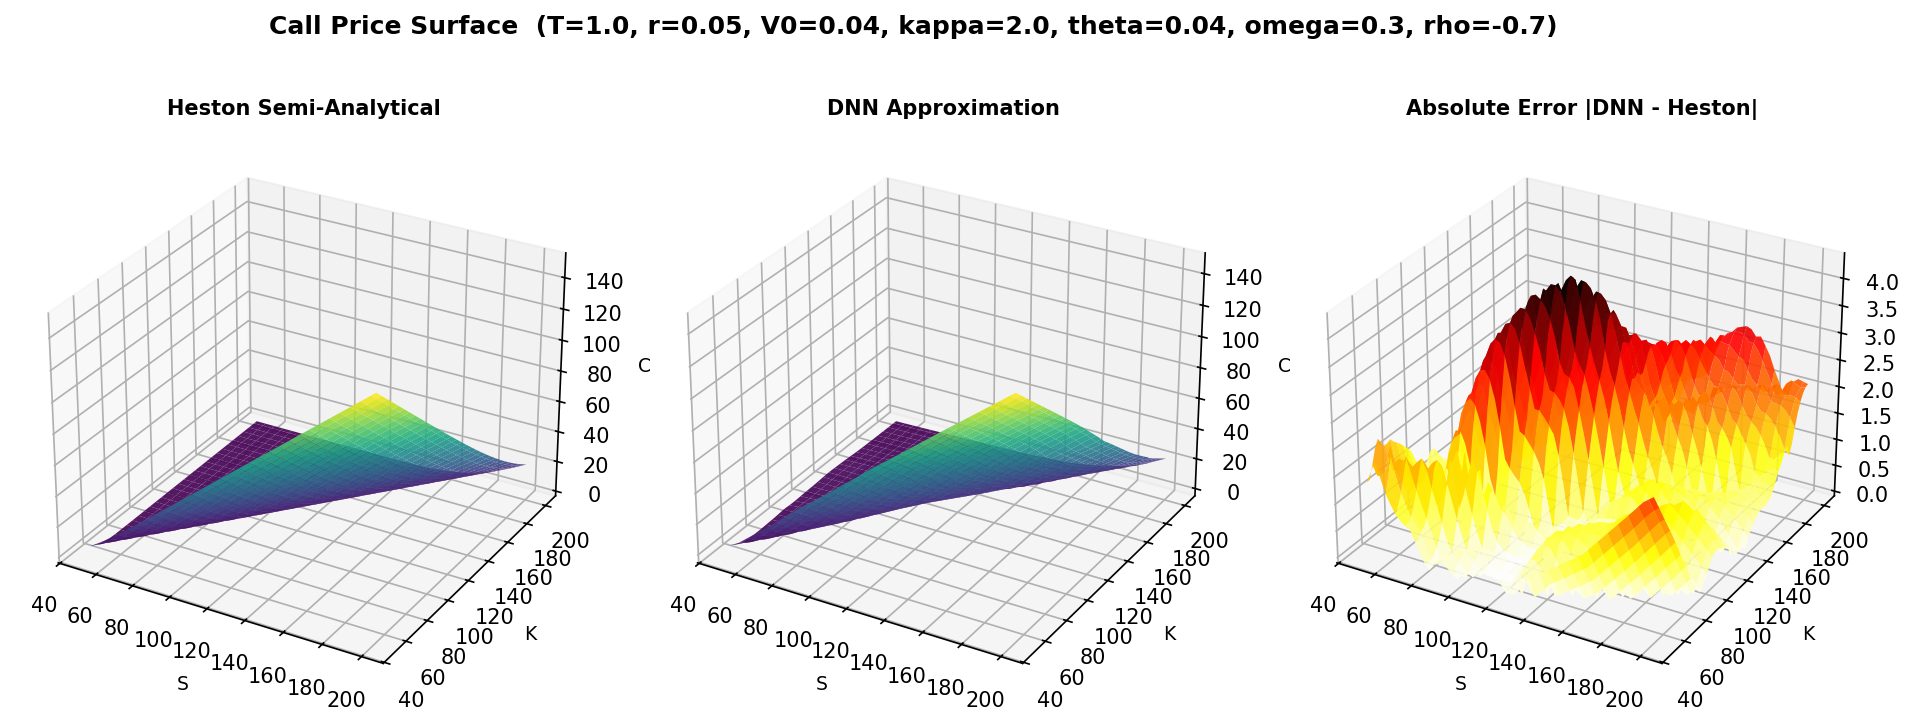
\includegraphics[width=0.95\textwidth]{figures/heston_pricing_surface.png}
    \caption{Heston call price as a function of $(S, K)$, with $T = 1$, $r = 0.05$, $V_0 = 0.04$, $\kappa = 2.0$, $\theta = 0.04$, $\omega = 0.30$ and $\rho = -0.70$ held fixed: the semi-analytic surface (left), the DNN's predicted surface (centre), and their absolute difference $|\hat C - C|$ (right).}
    \label{fig:dnn_heston_surface}
\end{figure}

The story is much the same as in Chapter 1, almost reassuringly so: the semi-analytic and DNN surfaces are visually close to indistinguishable, correctly capturing the overall convex shape and the way the price decays as $K$ grows relative to $S$, and the absolute error is concentrated overwhelmingly in the same deep out-of-the-money corner where the true price itself is smallest. The largest \emph{absolute} errors and the largest \emph{relative} errors continue to occur in the same place, the corner where the option is barely worth anything at all, which is exactly the mechanism behind the inflated mean relative error discussed above, now reappearing for a second, structurally different pricing model. Seeing the same qualitative pattern survive the jump from a five-parameter surface to a nine-parameter one is, if anything, good evidence that this is a genuine feature of how these surrogates behave near zero, rather than some quirk specific to the Black-Scholes setting.

\FloatBarrier

\bibliography{bibliography}
\end{document}